\chapter{Plataforma de desarrollo}
\label{cap:capitulo4}

\vspace{1cm}

En este capítulo se describen las plataformas de desarrollo utilizadas para la implementación del prototipo propuesto. En concreto, se detallan los componentes hardware empleados en la construcción del pastillero automatizado, así como las herramientas software utilizadas para su programación, diseño e interacción con el usuario. Todo ello se ha seleccionado siguiendo una filosofía de bajo coste, garantizando al mismo tiempo el correcto funcionamiento del sistema en tiempo real.\\

\section{Hardware}

En este apartado se describen los componentes hardware utilizados en el desarrollo del sistema. La selección de los elementos se ha realizado buscando siempre el bajo coste del dispositivo, priorizando componentes accesibles, fáciles de integrar y adecuados para un correcto funcionamiento en tiempo real.\\

El sistema se compone de un microcontrolador principal encargado del procesamiento y control, una interfaz de usuario basada en pantalla táctil resistiva, un sensor biomédico para la monitorización del pulso, así como la estructura física del pastillero diseñada mediante impresión 3D. Además, se incluyen los elementos necesarios para la comunicación inalámbrica y la alimentación del dispositivo.

\subsection{Microcontrolador ESP32-2432S028}

El núcleo del sistema está compuesto por un microcontrolador conocido como ESP32-2432S028, el cual se basa en el chip ESP32 y combina, dentro de un solo módulo, la capacidad de procesamiento, la comunicación inalámbrica y el control de periféricos.\\

Este microcontrolador destaca por incorporar conectividad WiFi y Bluetooth de forma nativa, lo que facilita la comunicación directa con la aplicación móvil sin requerir módulos adicionales. De este modo, disminuyen tanto el costo como la complejidad del sistema. Además, cómo se muestra en la Figura \ref{fig:esp32}, tiene suficientes pines \textit{General-Purpose Input/Output} (GPIO) para conectar sensores, actuadores y la pantalla táctil que viene incorporada.\\

\begin{figure}[H]
    \centering
    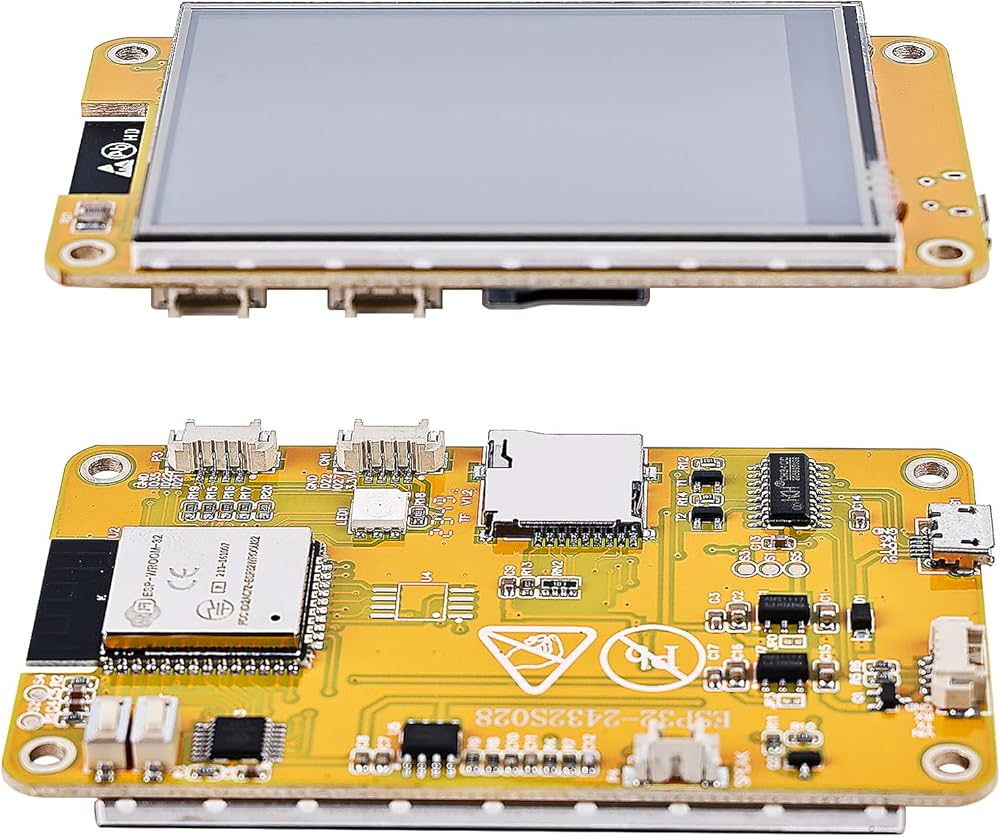
\includegraphics[width=0.5\textwidth]{figs/esp32.jpg}
    \caption{Microcontrolador ESP32-2432S028 utilizado en el sistema.}
    \label{fig:esp32}
\end{figure}

Una de las principales ventajas de este modelo es que incluye una pantalla TFT de 2.8 pulgadas con interfaz táctil resistiva, lo cual posibilita la integración de una interfaz para el usuario directamente en el dispositivo. Esto es importante para el proyecto ya que permite interactuar con el usuario sin tener que depender únicamente de la aplicación móvil.\\

En cuanto a su capacidad de procesamiento, el ESP32 cuenta con un procesador de doble núcleo que permite gestionar múltiples tareas de forma eficiente, como la lectura de sensores o la actualización de la interfaz gráfica. Más detalles sobre su configuración pueden consultarse en la Wiki del proyecto\footnote{\url{https://tinyurl.com/33n68ttv}}.

\subsubsection{Pantalla táctil}

La pantalla táctil resistiva que viene integrada en el microcontrolador constituye el principal medio de interacción directa entre el usuario y el dispositivo. El uso de una pantalla táctil permite mostrar información relevante de forma clara e intuitiva, como recordatorios de medicación, estados del sistema o lecturas del sensor biomédico. Asimismo, posibilita la interacción directa mediante pulsaciones, evitando la necesidad de botones físicos adicionales y simplificando el diseño del dispositivo.\\

Además, una interfaz táctil resistiva es más económica frente a otro tipo de tecnologías como podría ser la capacitiva, lo que hace que el dispositivo sea de bajo coste y más resistente en entornos domésticos. Por otro lado, teniendo en cuenta el perfil del usuario que emplearía este sistema, las pantallas táctiles resistivas presentan la ventaja de poder ser usadas con cualquier objeto o incluso con guantes.\\

Desde el punto de vista del diseño de la interfaz, se ha priorizado la simplicidad y la claridad visual, empleando elementos gráficos de gran tamaño y fácil identificación. Esto facilita el uso del dispositivo por parte de personas mayores o con poca experiencia en el uso de tecnologías digitales.\\

En conjunto, la pantalla táctil no solo actúa como elemento de visualización, sino que constituye un componente fundamental para mejorar la accesibilidad y la usabilidad del sistema.

\subsection{Sensor de pulso y SpO2}

Para monitorizar los parámetros biomédicos del usuario, se ha utilizado un sensor MAX30102. Este sensor permite medir de forma no invasiva tanto la frecuencia cardíaca como el nivel de oxigenación en sangre, siendo ampliamente utilizado en dispositivos portátiles de salud. En el presente proyecto se ha empleado principalmente para la estimación de la frecuencia cardíaca del usuario.

\begin{figure}[H]
    \centering
    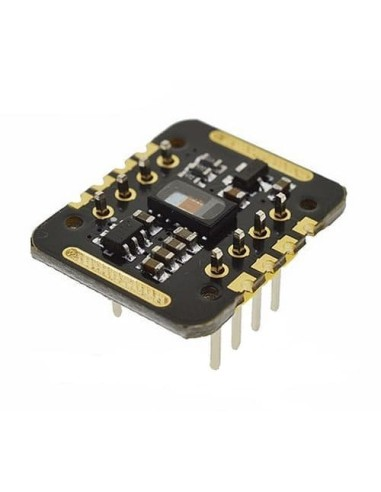
\includegraphics[width=0.35\textwidth]{figs/max30102.jpg}
    \caption{Sensor MAX30102 utilizado para la medición de pulso y SpO2.}
    \label{fig:max30102}
\end{figure}

El funcionamiento del sensor se basa en emitir luz a través de la piel, normalmente en longitudes de onda roja e infrarroja, midiendo la variación de la luz absorbida por la sangre. A partir de estas mediciones, es posible estimar tanto el pulso como la saturación de oxígeno.\\

Como se puede observar en la Figura \ref{fig:max30102}, el sensor presenta un tamaño reducido y una fácil integración con sistemas embebidos, lo que lo hace especialmente adecuado para aplicaciones portátiles y de bajo consumo.\\

La comunicación con el microcontrolador se realiza mediante el protocolo \textit{Inter-Integrated Circuit} (I2C), lo que permite una conexión sencilla utilizando un número reducido de pines. La incorporación de este sensor en el sistema permite añadir una funcionalidad adicional de seguimiento de la salud del usuario, complementando el objetivo principal del pastillero automatizado y aportando un mayor valor al dispositivo.

\subsection{Diseño mecánico del sistema}

El diseño mecánico del sistema se ha centrado en el desarrollo de un pastillero automatizado que permita almacenar y dispensar medicamentos de forma organizada, accesible y segura en un entorno doméstico. Para ello, se ha diseñado una estructura compacta que integra los distintos componentes del sistema, como el microcontrolador, el sensor biomédico y la interfaz de usuario.

\begin{figure}[H]
  \centering
  \begin{minipage}[t]{0.45\textwidth}
    \centering
    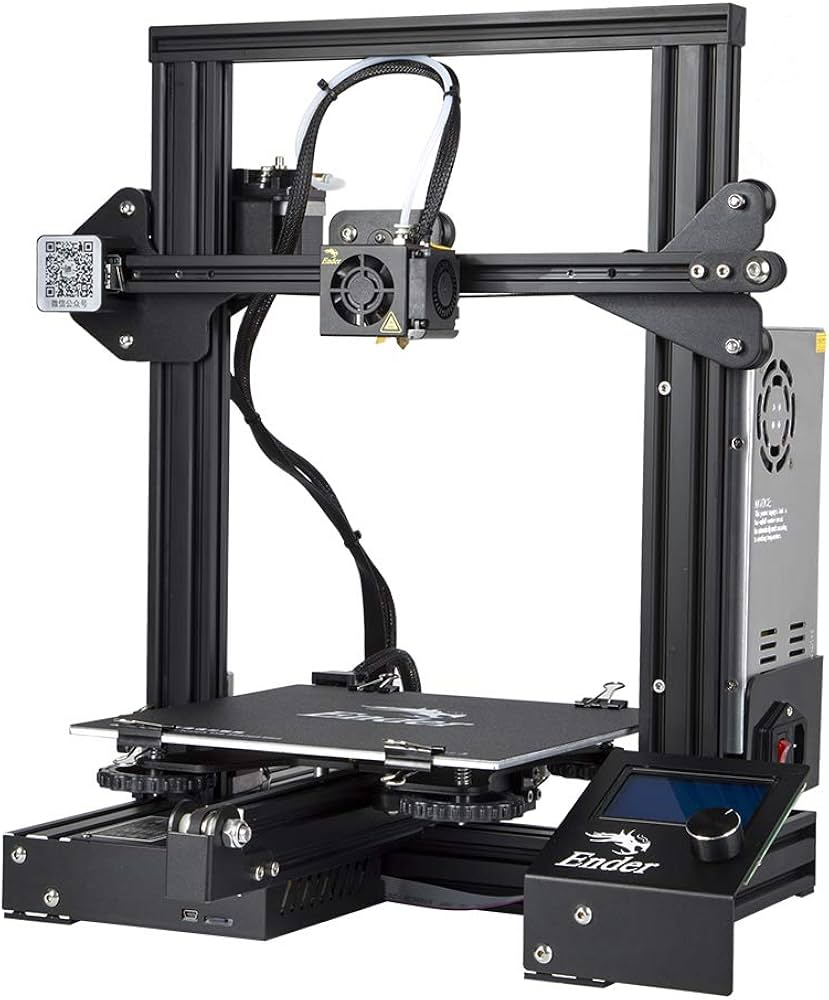
\includegraphics[height=7.15cm,width=5.75cm]{figs/ender3.jpg}

    \small a) Creality Ender 3, más asequible, menor calidad de impresión.
  \end{minipage}
  \hfill
  \begin{minipage}[t]{0.45\textwidth}
    \centering
    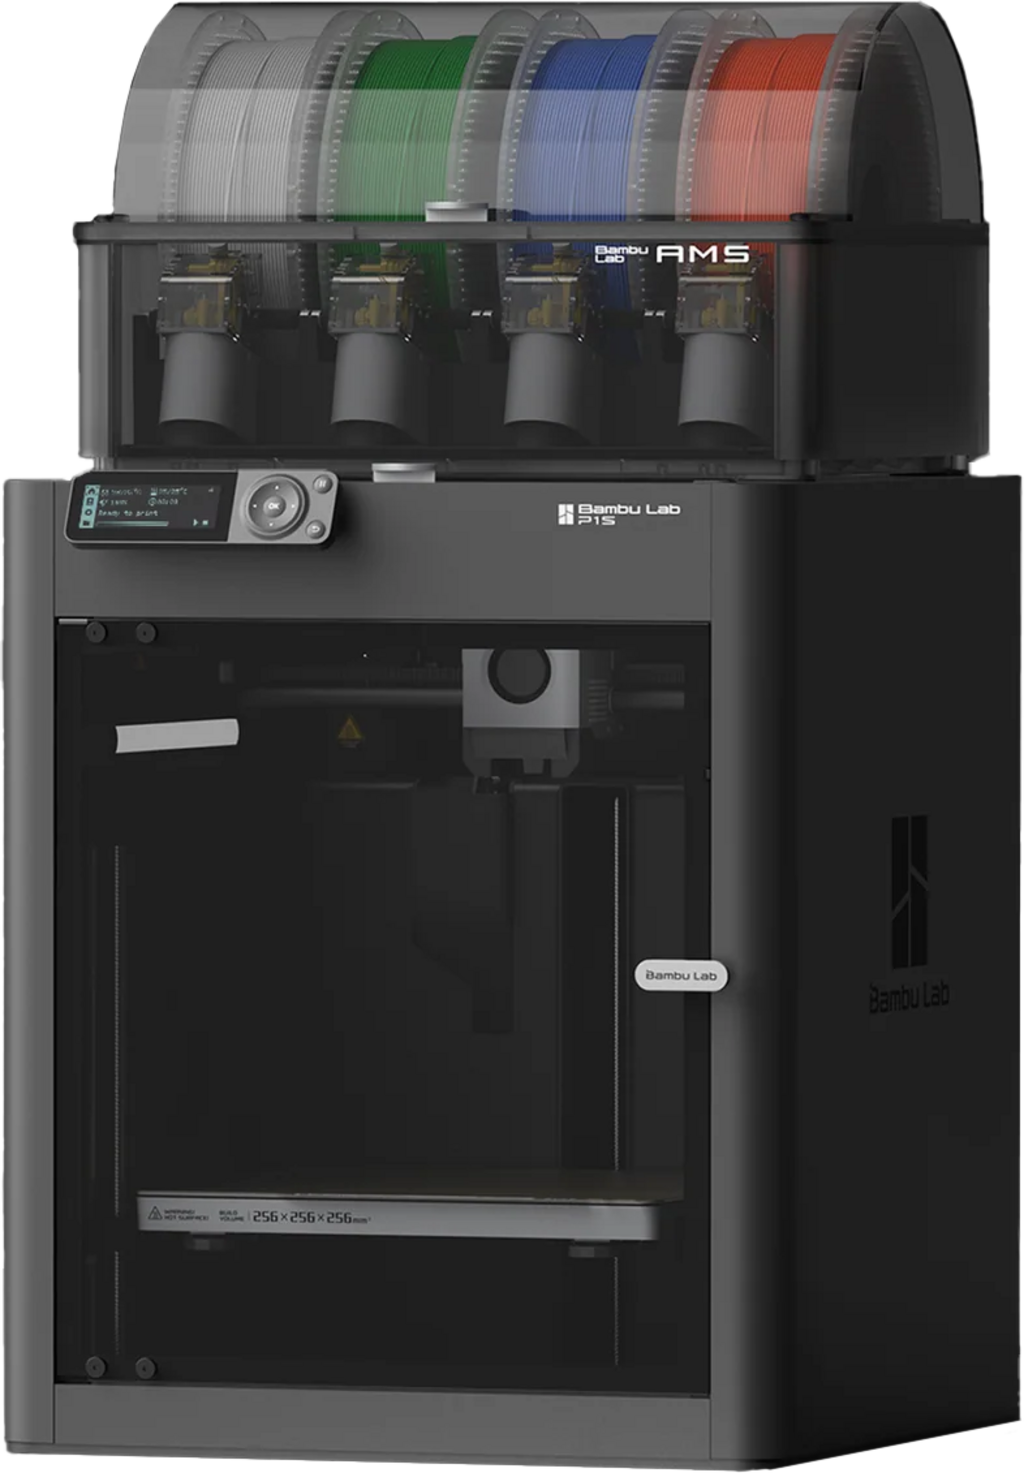
\includegraphics[height=7.15cm,width=5.75cm]{figs/bambulab.png}

    \small b) Bambu Lab P1S Combo, mayor precio, mayor calidad y multicolor.
  \end{minipage}

  \caption{Impresoras empleadas para imprimir el diseño mecánico del sistema.}
  \label{fig:impresoras}
\end{figure}

El modelado del dispositivo se ha realizado en 3D, lo que ha permitido definir con precisión la disposición de los componentes y realizar iteraciones del diseño hasta alcanzar una solución funcional y ergonómica. Se ha priorizado la facilidad de uso, empleando una disposición que facilite tanto la interacción con la pantalla como el acceso a los compartimentos de medicación.\\

La fabricación de las piezas se ha llevado a cabo mediante impresión 3D utilizando filamento \textit{Polylactic Acid} (PLA), seleccionado por su bajo coste y facilidad de uso en prototipado. Para ello, se han empleado dos impresoras distintas: una Creality Ender 3 y una Bambu Lab P1S Combo como las de la Figura~\ref{fig:impresoras}. El uso de ambas ha permitido observar diferencias en la calidad de impresión, especialmente en la precisión dimensional y el acabado superficial, lo que influye en el ajuste entre piezas y en el resultado final del dispositivo.\\

Finalmente, el diseño se ha planteado de forma modular, permitiendo de esta manera futuras modificaciones o ampliaciones del sistema sin necesidad de rediseñar completamente la estructura.

\subsection{Sistema de actuación}

El sistema de actuación del dispositivo es el encargado de realizar la dispensación de la medicación, permitiendo el avance controlado de los compartimentos del pastillero en función de las tomas programadas. Para ello, se ha empleado un servomotor modelo SG90 como el de la Figura~\ref{fig:sg90}, seleccionado por su bajo coste, tamaño reducido y facilidad de control mediante señales \textit{Pulse Width Modulation} (PWM) desde el microcontrolador.\\

\begin{figure}[H]
    \centering
    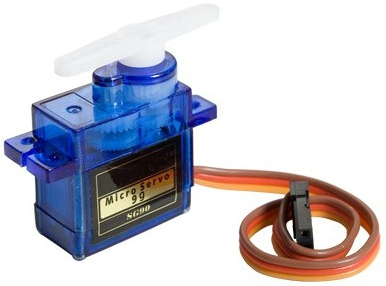
\includegraphics[width=0.45\textwidth]{figs/sg90.jpg}
    \caption{Servomotor SG90 empleado como actuador del sistema.}
    \label{fig:sg90}
\end{figure}

Para transformar el movimiento del servomotor en un desplazamiento discreto y controlado de los compartimentos, se ha diseñado un mecanismo basado en un sistema de trinquete accionado mecánicamente. Este tipo de mecanismo permite convertir el movimiento angular del servomotor en avances secuenciales del carrusel, garantizando que cada compartimento quede correctamente posicionado para la dispensación de la medicación.\\

El sistema está compuesto por un elemento impulsor conectado al servomotor, un mecanismo de trinquete encargado de producir el avance del carrusel y un sistema de bloqueo asistido por muelle. La Figura~\ref{fig:trinquete} muestra el conjunto de piezas diseñadas para implementar este mecanismo. Durante el funcionamiento, el impulsor transmite el movimiento generado por el servomotor al carrusel, produciendo un avance controlado de una posición en cada actuación. Tras completar el movimiento, el sistema recupera su posición inicial gracias a la acción del muelle, quedando preparado para el siguiente accionamiento.\\

El sistema de bloqueo impide movimientos involuntarios entre posiciones consecutivas, asegurando que el carrusel permanezca estable una vez completado cada avance. De este modo, cada activación del servomotor produce un único desplazamiento controlado, permitiendo una dispensación fiable y repetible.\\

\begin{figure}[H]
\centering
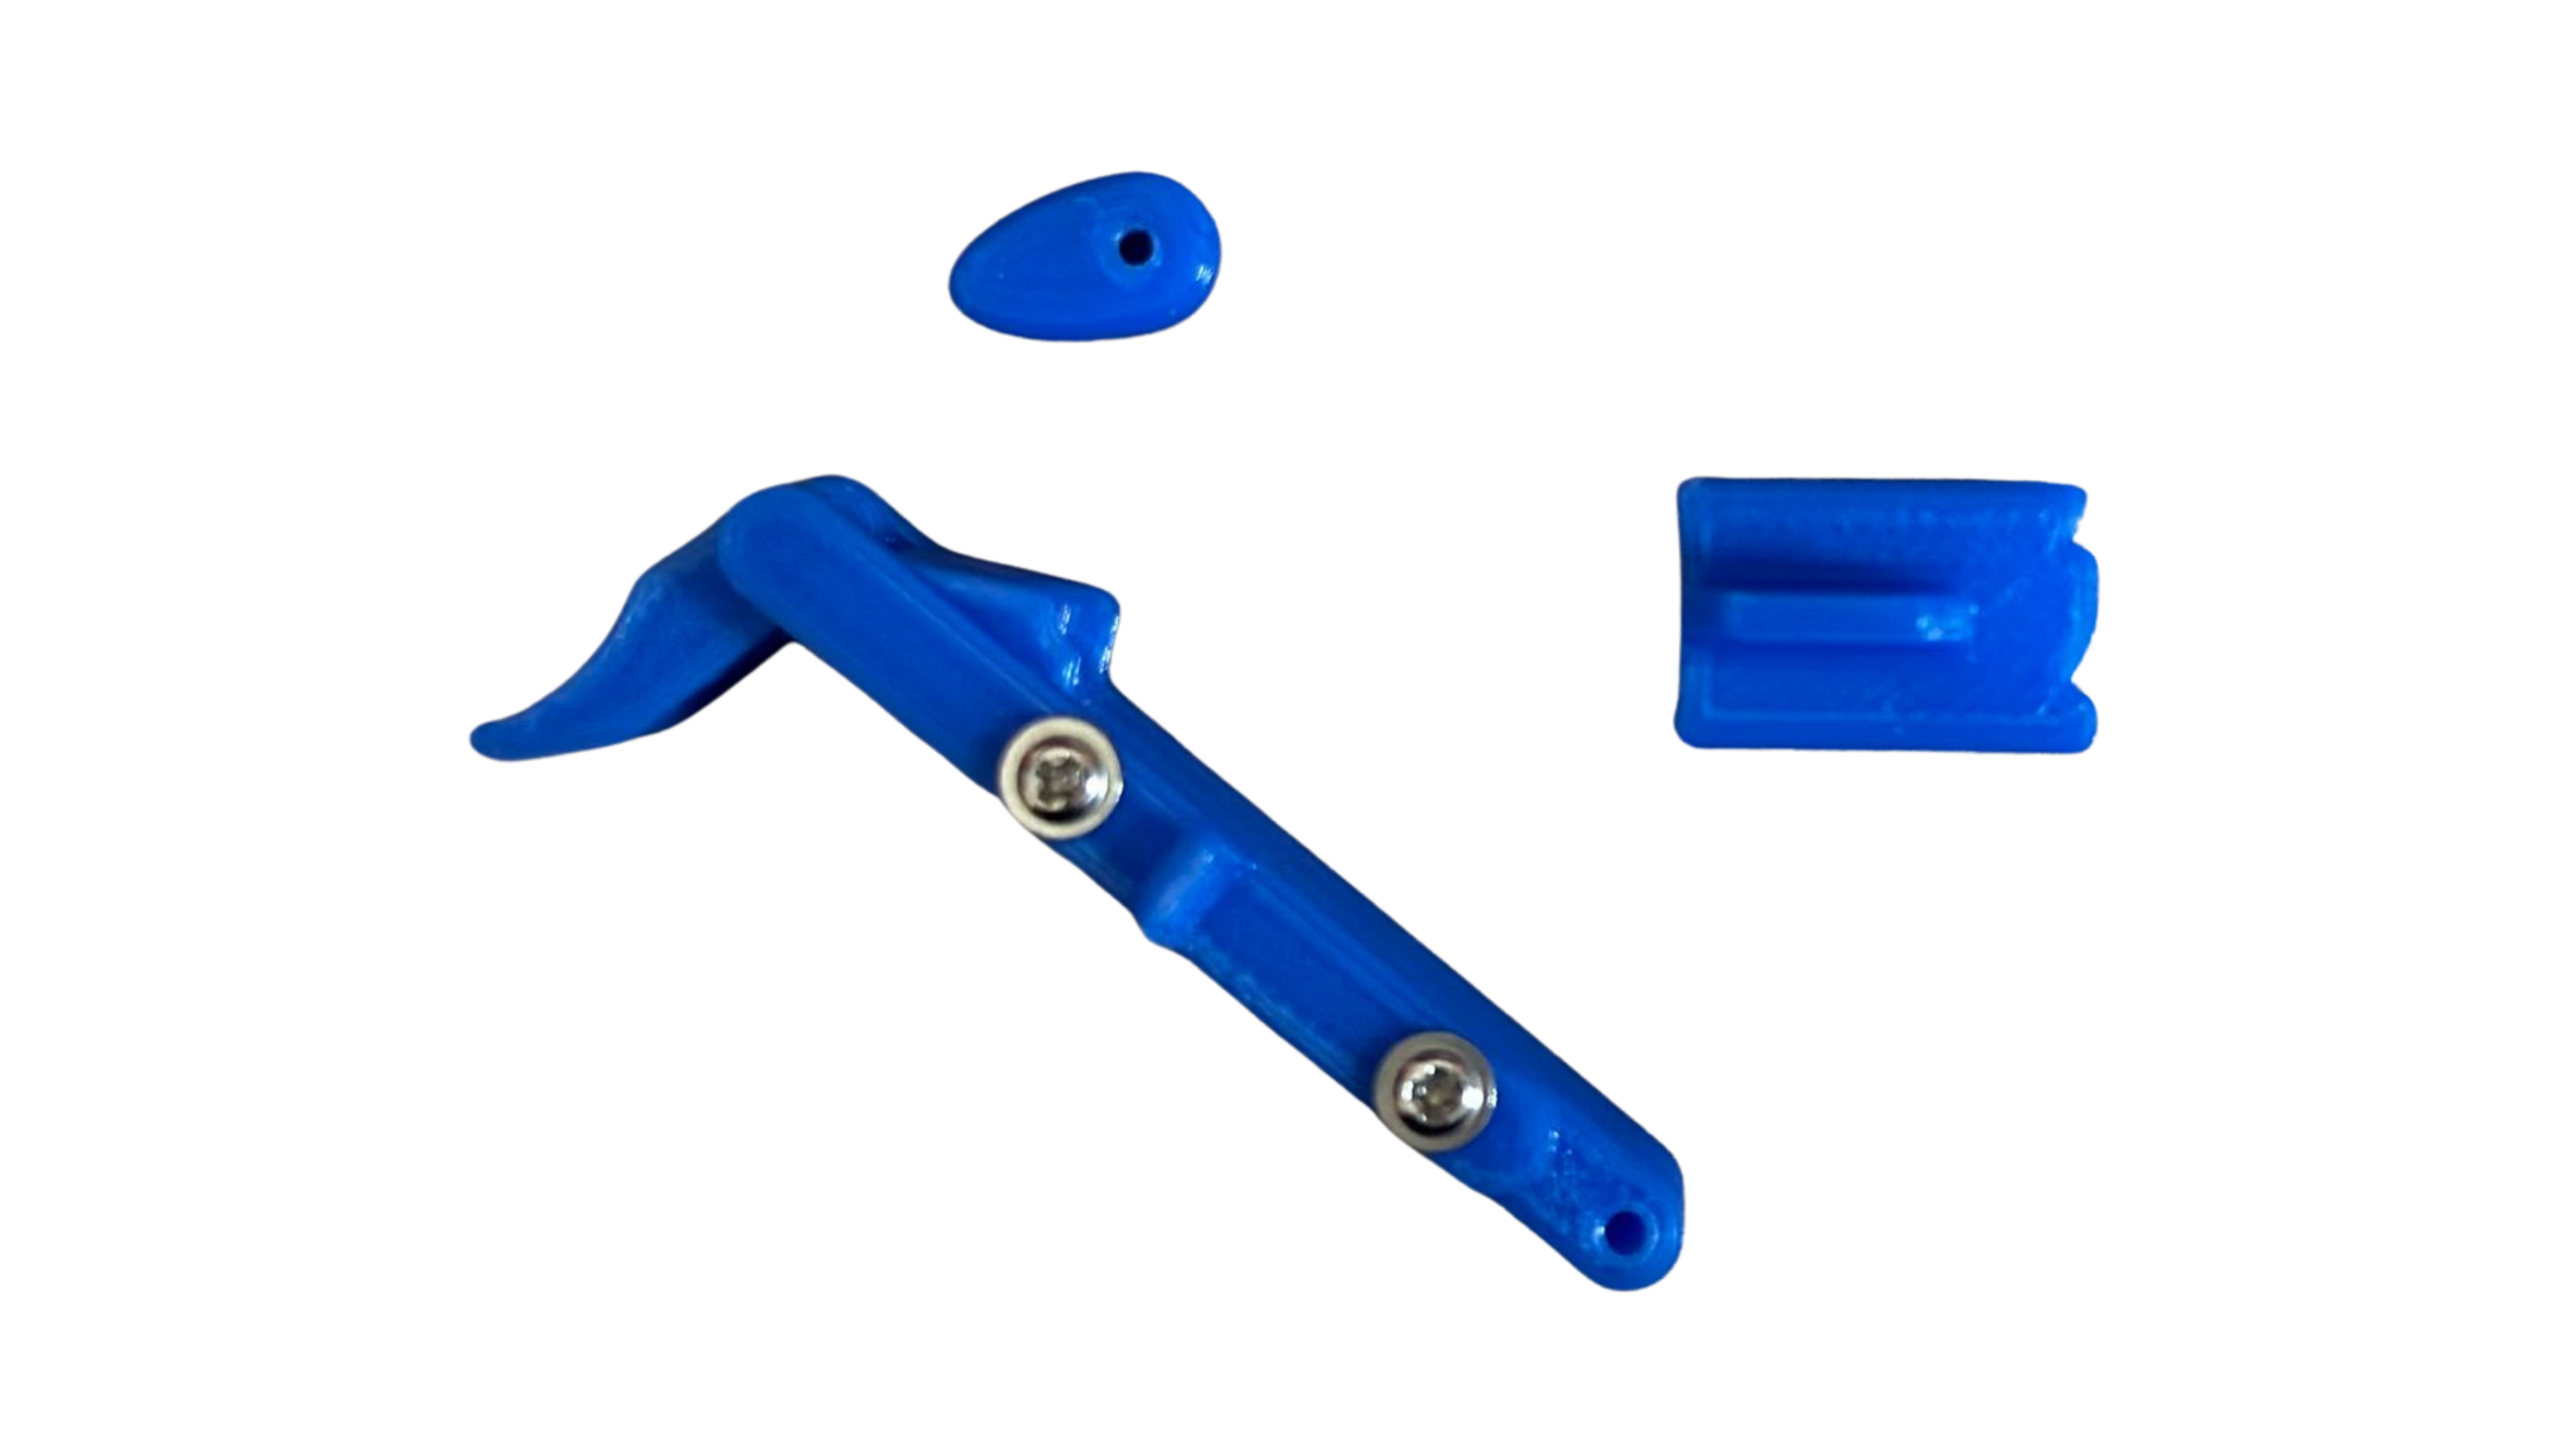
\includegraphics[width=0.65\textwidth]{figs/Trinquete_mecanismo.png}
\caption{Partes del mecanismo de trinquete utilizado en el sistema de dispensación.}
\label{fig:trinquete}
\end{figure}

Este enfoque permite obtener un sistema mecánico sencillo, robusto y fácilmente fabricable mediante impresión 3D, reduciendo la complejidad del conjunto y garantizando un posicionamiento adecuado de los compartimentos durante el funcionamiento del dispositivo.

\subsection{Sistema de aviso}

El dispositivo incorpora un sistema de aviso sonoro con el objetivo de notificar al usuario la toma de medicación de forma clara e inmediata. Para ello, se ha utilizado un altavoz de 4\si{\ohm} y 3\si{\watt} como el de la Figura~\ref{fig:altavoz}, conectado al microcontrolador.\\

\begin{figure}[H]
    \centering
    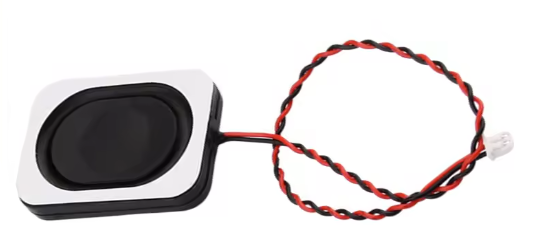
\includegraphics[width=0.7\textwidth]{figs/altavoz.png}
    \caption{Altavoz empleado en el sistema para avisos sonoros.}
    \label{fig:altavoz}
\end{figure}

\

Este sistema permite complementar las alertas visuales mostradas en la pantalla táctil, mejorando la accesibilidad del dispositivo, especialmente en situaciones en las que el usuario no esté prestando atención directa a la interfaz o presente dificultades visuales.\\

El control del altavoz se realiza desde el microcontrolador, que genera señales acústicas en los momentos programados para cada toma. De este modo, se garantiza que el usuario reciba un aviso tanto visual como sonoro, aumentando la fiabilidad del sistema.\\

\subsection{Electrónica de integración}

Para organizar de forma estructurada las conexiones entre el microcontrolador, los actuadores y los sensores, se ha diseñado una placa de circuito impreso específica. La \textit{Printed Circuit Board} (PCB) incorpora un controlador PWM basado en el circuito integrado PCA9685, el cual permite gestionar múltiples servomotores mediante comunicación I2C con el microcontrolador. Esto facilita el control simultáneo de varios actuadores, reduciendo la carga de procesamiento y simplificando la generación de señales PWM.\\

Asimismo, la placa incluye los elementos necesarios para la correcta alimentación del sistema, como los condensadores, destacando uno de \SI{1000}{\micro\farad} que contribuye a estabilizar la tensión de alimentación y evitar caídas de voltaje durante el funcionamiento de los servomotores.

\begin{figure}[H]
    \centering
    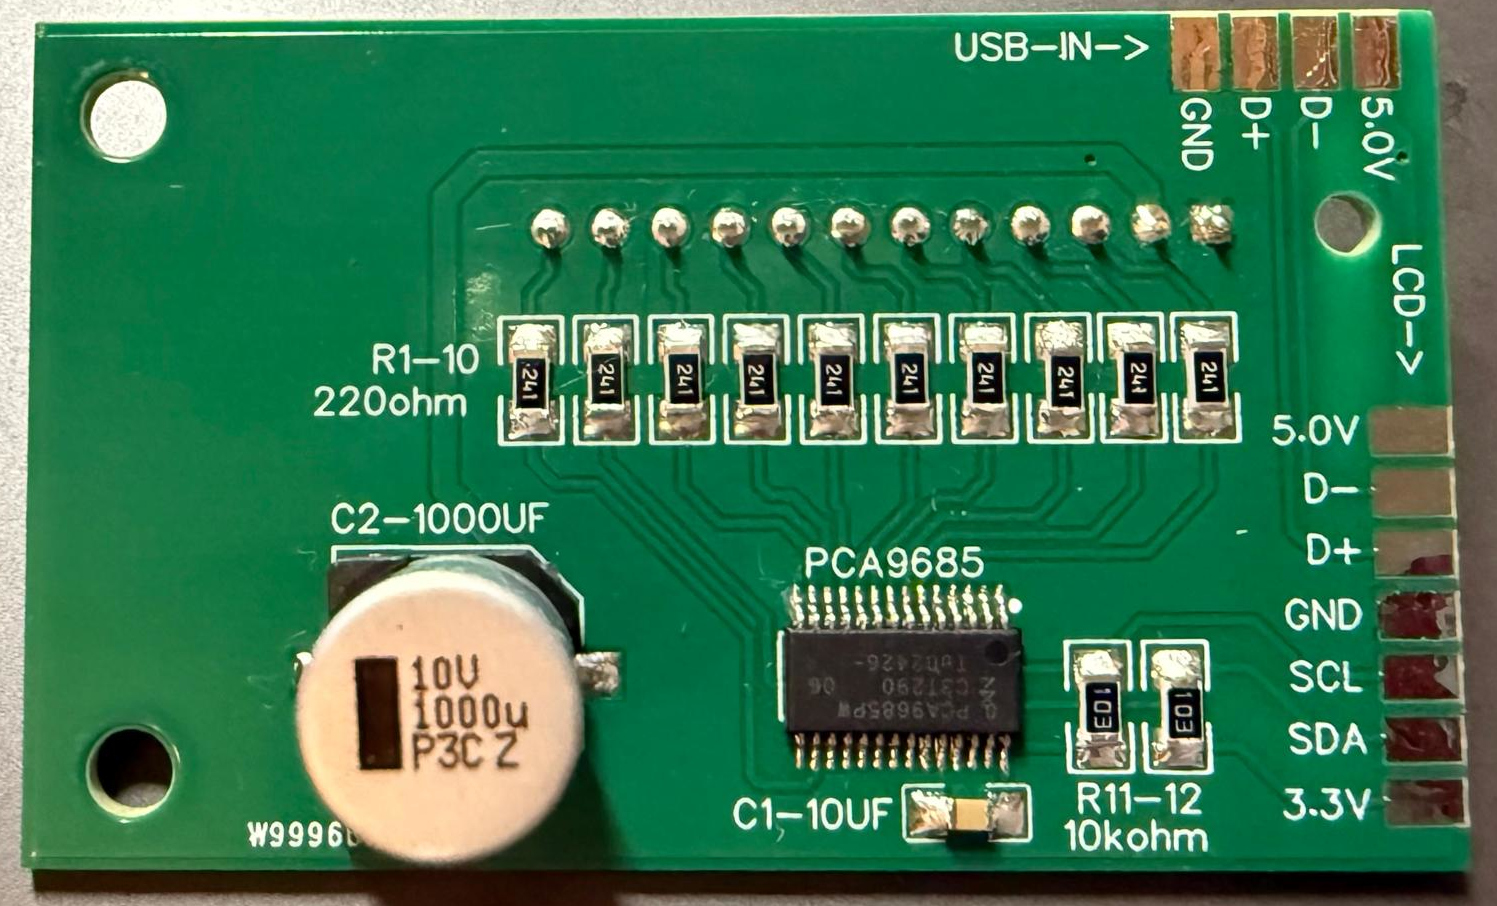
\includegraphics[width=0.55\textwidth]{figs/pcb.jpeg}
    \caption{Placa de circuito impreso (PCB) utilizada para la integración del sistema.}
    \label{fig:pcb}
\end{figure}

La comunicación con el microcontrolador se realiza mediante el protocolo I2C, utilizando las líneas SDA y SCL, junto con resistencias \textit{pull-up} integradas en la propia PCB. Además, se han dispuesto las conexiones necesarias para la alimentación a \SI{5}{\volt} y \SI{3.3}{\volt}, así como las salidas correspondientes para el control de los actuadores.\\

Como se muestra en la Figura~\ref{fig:pcb}, el diseño de la PCB permite una integración compacta y organizada de todos los elementos electrónicos; de este modo, se reduce el cableado y se mejora la fiabilidad del sistema. La alimentación se realiza a través de un conector USB tipo C integrado en la propia PCB, que proporciona una tensión de \SI{5}{\volt}, simplificando el diseño y reduciendo el número de conexiones externas.


\section{Software}
En este apartado se describen las herramientas software utilizadas para el desarrollo del sistema, abarcando tanto el \textit{firmware} del microcontrolador como la aplicación móvil y el diseño de los componentes mecánicos.\\

Cada una de estas herramientas ha sido empleada en un ámbito específico del proyecto, permitiendo así implementar las distintas funcionalidades del sistema de forma estructurada. En concreto, se han utilizado \textit{PlatformIO} para el desarrollo del \textit{firmware} del dispositivo, \textit{Android Studio} para la creación de la aplicación móvil y \textit{Sharp3D} para el diseño de las piezas del sistema.

\subsection{PlatformIO}

Para el desarrollo del \textit{firmware} del microcontrolador se ha utilizado \textit{PlatformIO} como entorno de desarrollo, empleando el lenguaje de programación C++. Esta herramienta facilita la gestión de librerías, la compilación del código y su implementación de manera eficaz en el ESP32.\\

Además, como se muestra en la Figura~\ref{fig:platformio}, PlatformIO permite trabajar con múltiples dependencias de manera organizada, lo que resulta especialmente útil en proyectos de sistemas embebidos. En este caso, se ha utilizado junto con la librería LVGL (\textit{Light and Versatile Graphics Library}) para el desarrollo de la interfaz gráfica en la pantalla táctil.\\

\begin{figure}[H]
    \centering
    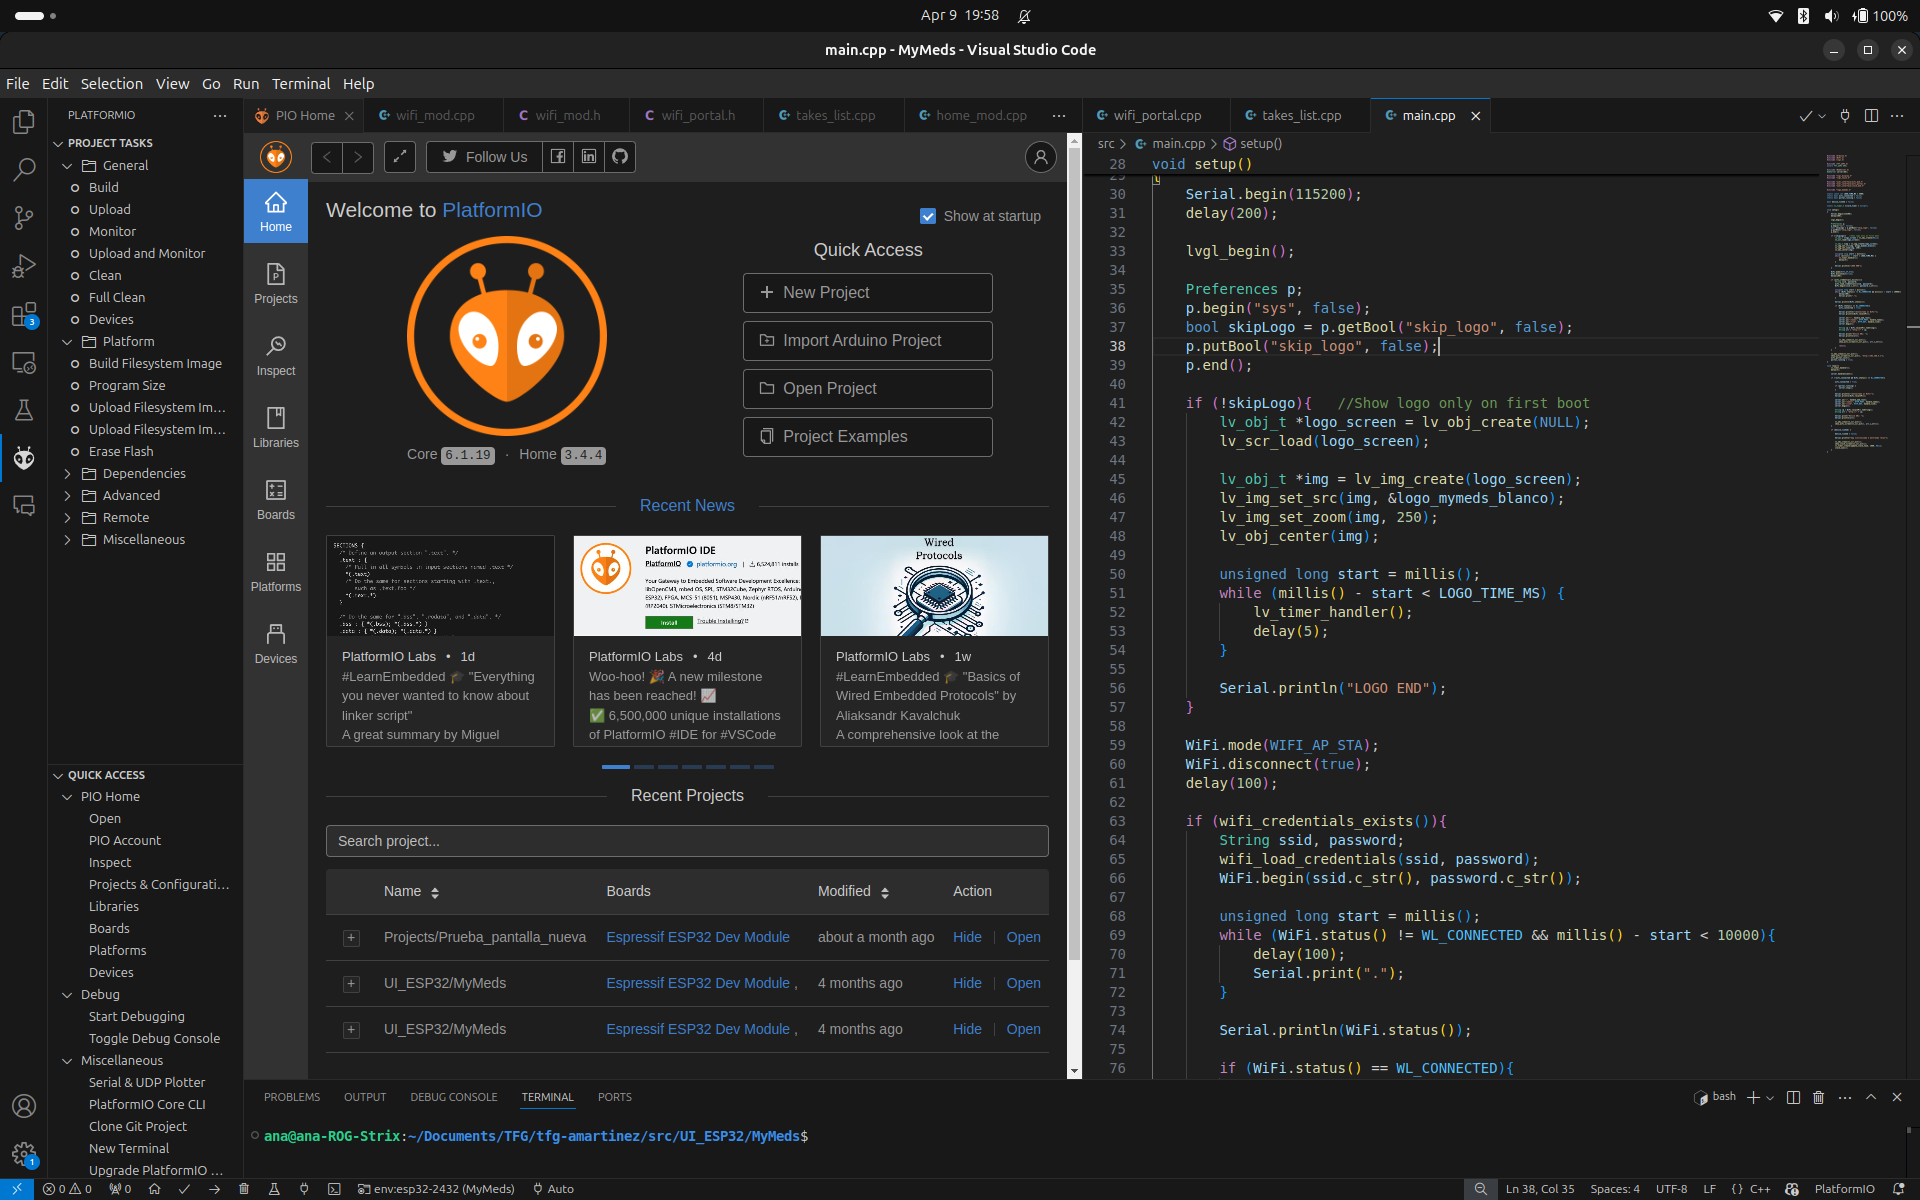
\includegraphics[width=\textwidth]{figs/platformio.png}
    \caption{Entorno de desarrollo \textit{PlatformIO} utilizado para la programación del microcontrolador.}
    \label{fig:platformio}
\end{figure}

El \textit{firmware} implementado se encarga del control de los servomotores, la lectura de datos del sensor biomédico y la gestión de la interfaz de usuario, garantizando un funcionamiento en tiempo real del sistema.\\

\subsection{Android Studio}

La aplicación móvil ha sido desarrollada utilizando \textit{Android Studio} como entorno de desarrollo, empleando el lenguaje de programación \textit{Kotlin}. Esta herramienta proporciona un entorno completo para el diseño, desarrollo y depuración de aplicaciones Android.\\

Además, \textit{Android Studio} permite probar la aplicación tanto mediante emulación en un dispositivo virtual integrado en el propio entorno (parte derecha de la Figura~\ref{fig:app}), como en un dispositivo móvil físico. Esto ha facilitado la validación del funcionamiento de la aplicación en distintas condiciones de uso.\\

\begin{figure}[H]
    \centering
    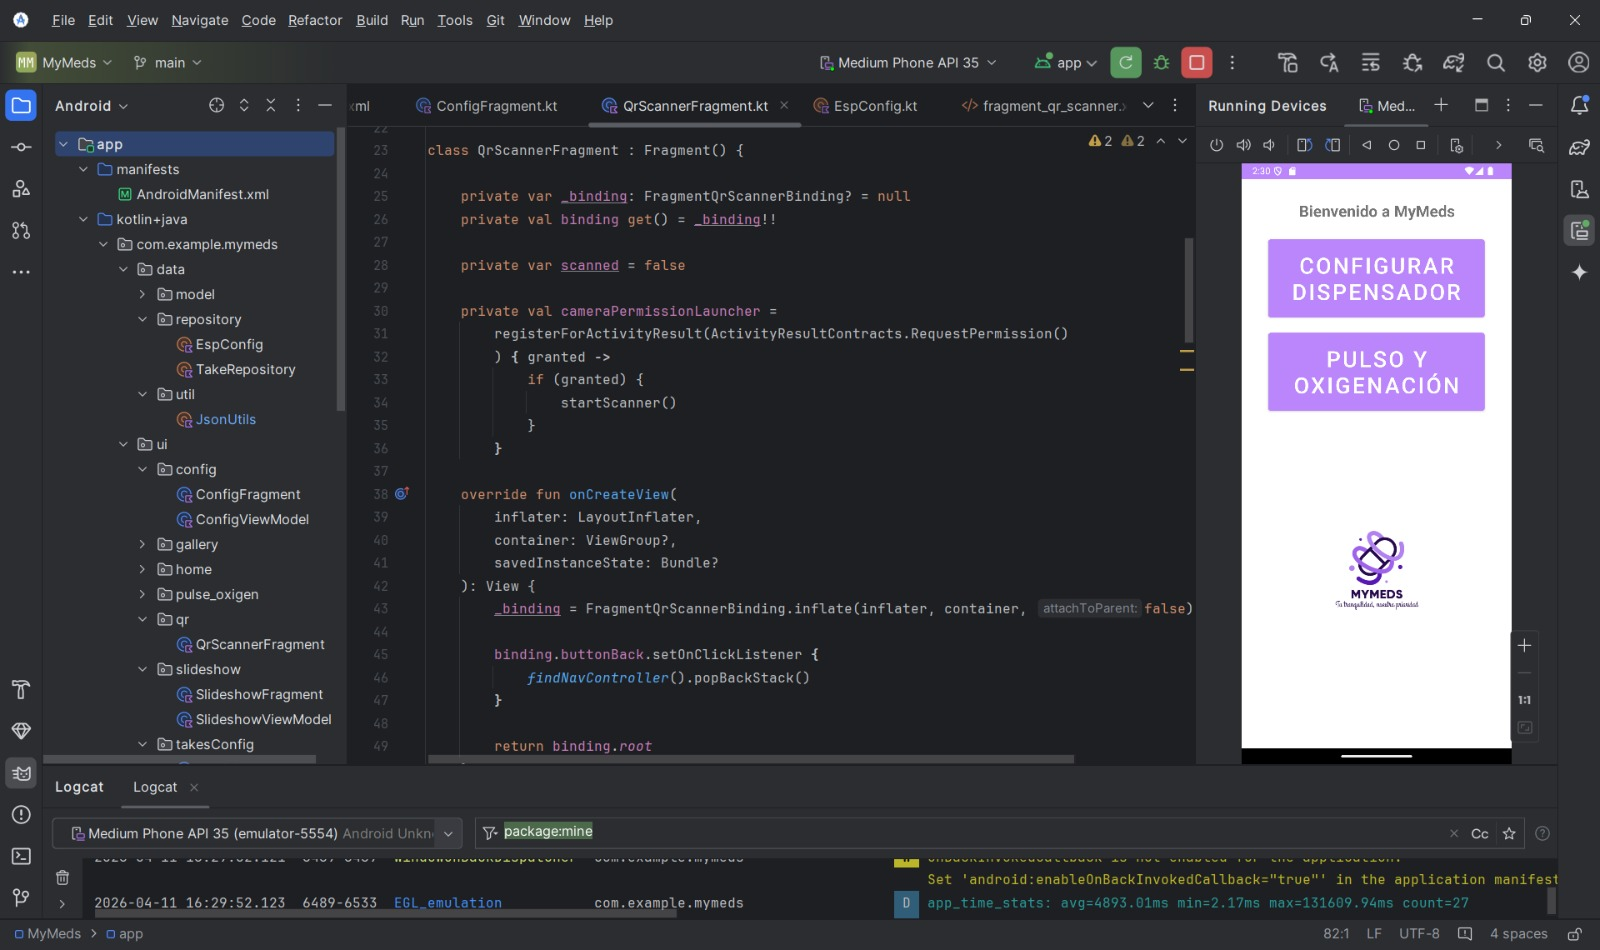
\includegraphics[width=\textwidth]{figs/app.jpeg}
    \caption{Aplicación móvil desarrollada en \textit{Android Studio}.}
    \label{fig:app}
\end{figure}

La aplicación implementada permite al usuario configurar el dispositivo, gestionar la medicación y consultar el historial de datos recogidos por el sensor biomédico. Para ello, se ha diseñado una interfaz sencilla e intuitiva, priorizando la accesibilidad y la facilidad de uso. Como se muestra en el entorno de emulación de la Figura~\ref{fig:app}, la interfaz ha sido diseñada de forma sencilla e intuitiva.\\

De esta forma, la aplicación actúa como complemento del sistema físico, permitiendo una interacción remota y mejorando la experiencia de usuario.

\subsection{Sharp3D}

Para el diseño de los componentes mecánicos del sistema se ha utilizado el software \textit{Sharp3D}, una herramienta de modelado 3D que permite crear y modificar piezas de forma precisa.\\

Mediante esta aplicación se han diseñado las distintas partes del pastillero, incluyendo la estructura principal y los elementos móviles necesarios para el funcionamiento del sistema. Como se muestra en la Figura~\ref{fig:sharp3d}, el modelo 3D permite visualizar y ajustar el diseño antes de su fabricación. Estos modelos han sido posteriormente exportados para su fabricación mediante impresión 3D.\\

\begin{figure}[H]
    \centering
    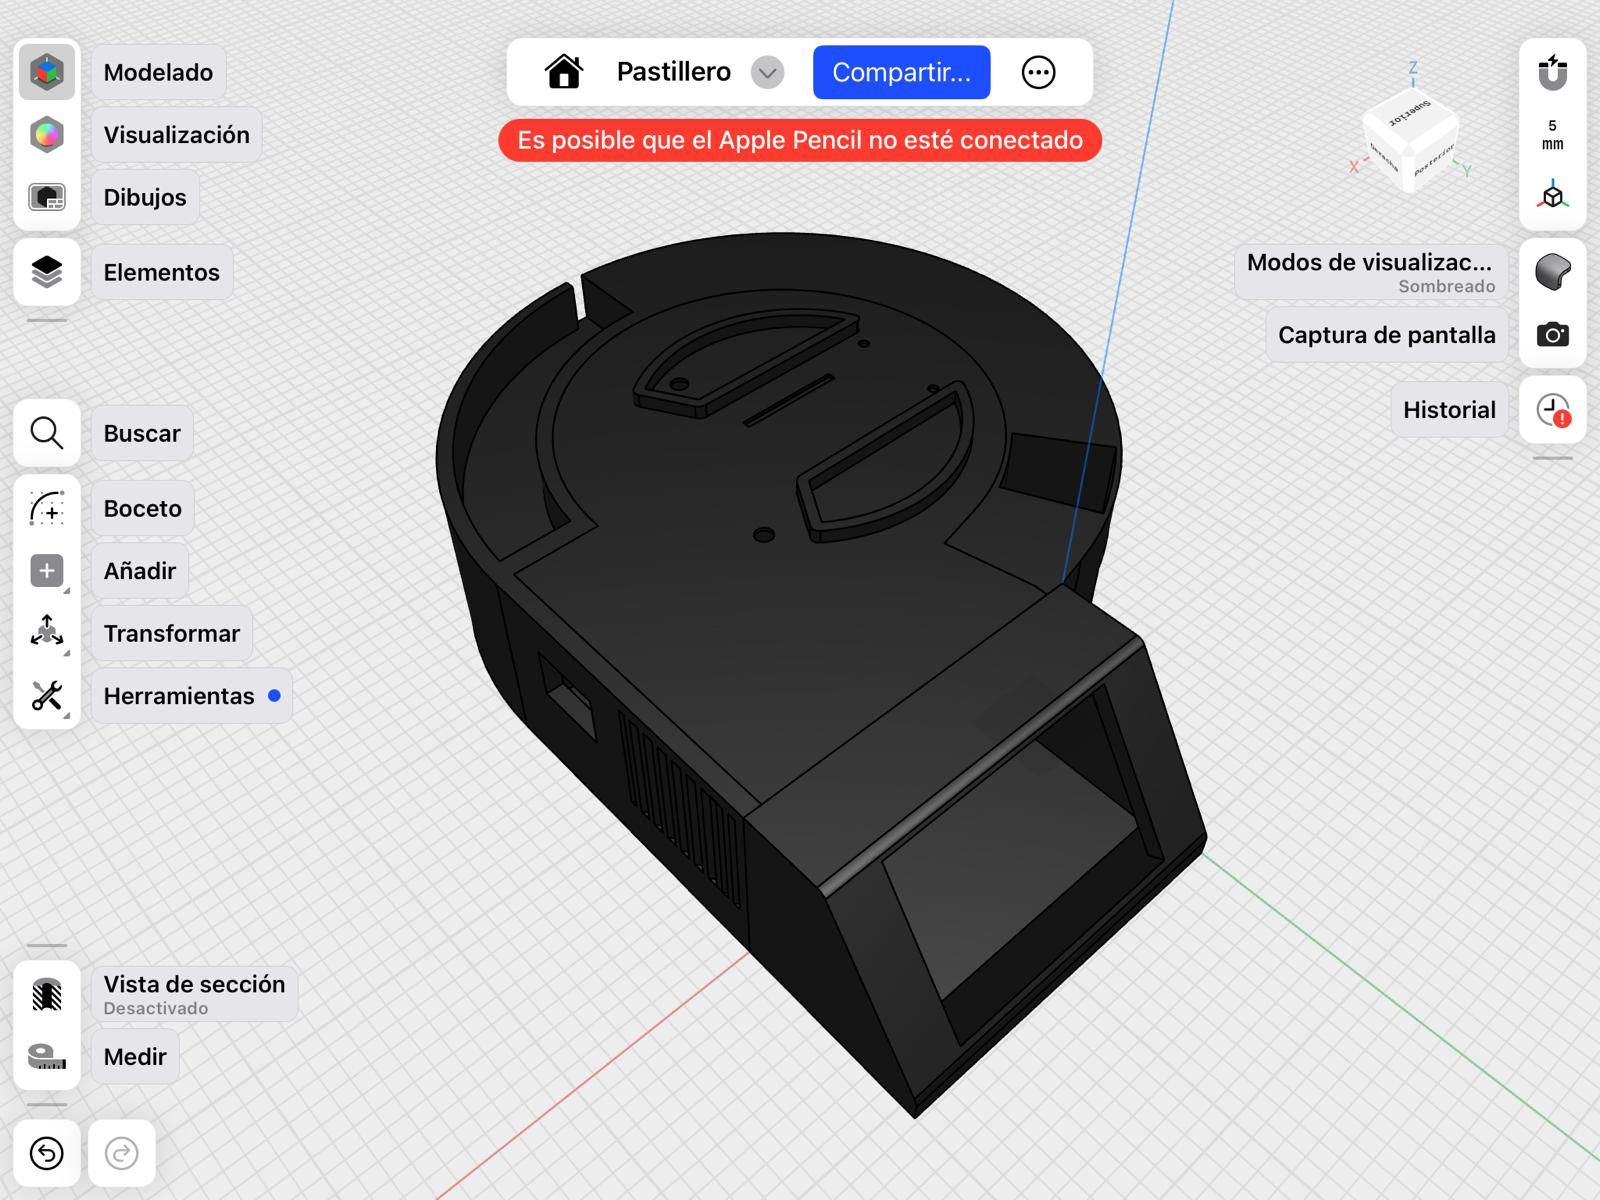
\includegraphics[width=\textwidth]{figs/3d.jpeg}
    \caption{Modelo 3D de la base del pastillero diseñado en \textit{Sharp3D}.}
    \label{fig:sharp3d}
\end{figure}

El uso de esta herramienta ha permitido adaptar el diseño del dispositivo a los requisitos del proyecto, facilitando de esta forma la iteración y mejora de las piezas hasta obtener una solución funcional.
